\chapter{Architectural Design}

\begin{figure}[htb!]
\centering%
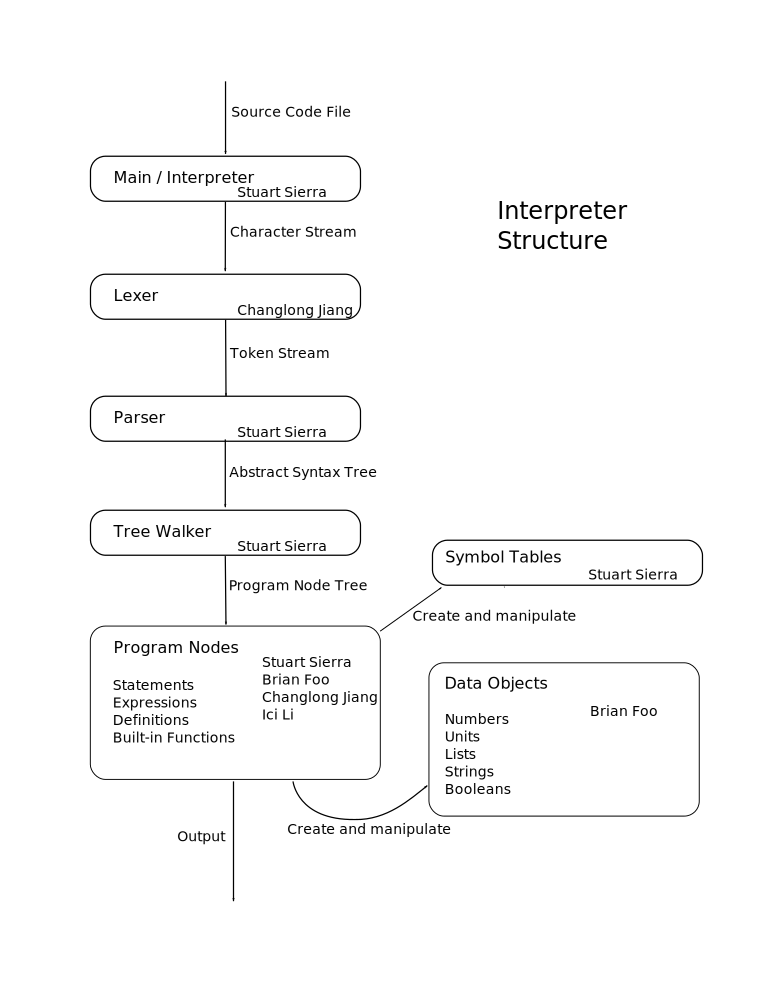
\includegraphics[width=1.0\textwidth]{structure}
\label{fig:structure}
\end{figure}

Physicalc is an interpreted programming language.  The diagram on
page~\pageref{fig:structure} shows the general structure of the
interpreter.  The lexer and parser produce an abstract syntax tree,
which is transformed by a tree walker into a tree of program nodes.
The program nodes are all sub-classes of the Node class, each node
represents a single program structure such as a statement or a
function call.  Every node class provides an ``eval'' method which is
responsible for executing the behavior of that node.

The root of a tree is an instance of the Program class.  The
interpreter calls ``eval'' on the Program, which calls ``eval'' on its
sub-nodes, and so on, recursively, so the node tree executes itself.
The symbol tables are carried through the tree as arguments to
``eval.''  Because Physicalc does not support nested scopes, there are
never more than two symbol tables, one global and one local, in effect
at any given time.  The node structure was designed by Stuart Sierra,
and the sub-classes were implemented by Ici Li and Changlong Jiang.

The data objects manipulated by a Physicalc program---numbers, units,
lists, and strings---are all sub-classes of the Datum class.  Datum
defines virtual methods for all the arithmetical operators, which are
overridden in sub-classes.  Calling an operator on two types for which
it is not defined, e.g.\ addition between two units, results in a
exception of class TypeError.  Brian Foo implemented the Datum
sub-classes.
